\itemhead{复习题三 · 第14题（教材p.91）}{XJ-B1-C03-RV-P091-Y1267}
\label{XJ-B1-C03-RV-P091-Y1267}
{\footnotesize 湘教版教材p.91 / PDF第98页 / 复习题三 / 第14题}
\field{原题}{某市对家庭每月用水的收费规定为：若用水量不超过基本月用水量 $a\,\mathrm{m^3}$，则只付基本费 8 元和损耗费 $c\ (c<5)$ 元；若用水量超过基本月用水量，则除了需付基本费和损耗费外，超过部分还需按 $b$ 元/$\mathrm{m^3}$ 进行付费。已知该市某家庭 1—3 月的用水量分别为 $9\,\mathrm{m^3},15\,\mathrm{m^3}$ 和 $22\,\mathrm{m^3}$，其支付的费用分别为 9 元、19 元和 33 元。试写出每月支付费用 $y$（元）关于月用水量 $x$（$\mathrm{m^3}$）的函数，并画出函数的图象。}
\field{参考答案}{$a=10,b=2,c=1$，故 $y=9$（$0\le x\le10$）、$y=2x-11$（$x>10$）。图象为水平线段与从 $(10,9)$ 向右上延伸的射线，两段在边界衔接。}
\begin{center}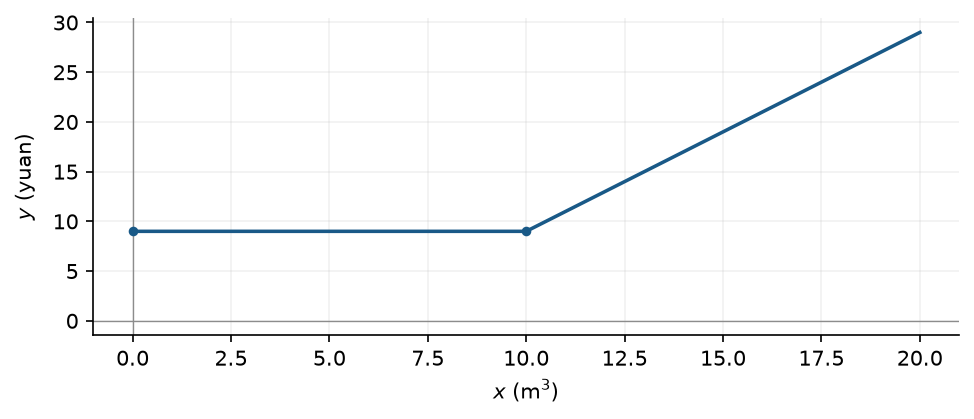
\includegraphics[width=.84\linewidth,height=.38\textheight,keepaspectratio]{figures/C03-RV091-14.png}\end{center}
{\small \field{关联知识}{F07 分段函数、绝对值及分段应用（教材帮p.86、91、92、93 / PDF95、100、101、102）；F03 函数求值、解析式与函数建模（教材帮p.80、87、88、89、90、131 / PDF89、96、97、98、99、140）}
\field{方法与易错点}{先列转折点和各段条件，再建立分段式，检查衔接、定义域与值域。 易错：跨段套公式；超额部分按全量收费；绝对值去号漏区间。}
\field{答案依据}{答案册相关题组：PDF第24、25、26、27页（册内页23、24、25、26）；按当前题库原题逐项重算，不按旧版题号机械对套。}}
